\documentclass{article}

\usepackage{nomencl}
\makenomenclature

\usepackage{amsthm} %Theorem package
\usepackage{amsmath} %
\usepackage{graphicx}
\usepackage{subfigure}
\usepackage{verbatim}
\usepackage{epstopdf}
\usepackage{booktabs}


\newtheorem{theorem}{Theorem}[section]
\newtheorem{corollary}[theorem]{Corollary}
\newtheorem{defination}{Definition}[section]
\newtheorem{proposition}{Proposition}[section]

\begin{document}
\nomenclature{MAC}{Message Authentication Code: A short message block generated
with message protected. MAC is concatenated to the rightmost of the message in
transmission}
\nomenclature{Tag}{The output short block of a MAC generation scheme}
\nomenclature{(M,T)}{Message M and its tag T}
\nomenclature{TG(M, $\ldots$)}{A MAC Scheme processing the message M with
secret information in the arguments list}
\nomenclature{VF(M,T, $\ldots$)}{Verify the message M and tag T with the secret
information in the arguments list. Return 1
if TG(M,$\ldots$) = T and 0 if not.}
\nomenclature{UF-CMA}{Unforgeability under adaptive Chosen Message Attack}
\nomenclature{Pr[A]}{The probability that event A happens}
\nomenclature{Forgery(MAC, A)}{Forgery experiment on a MAC scheme with the
adversary A. Return 1 if A succeed a forgery attack otherwise 0}
\nomenclature{Forgery$_{MAC}$}{The probability that Forgery(MAC, A)=1 for an
adversary A and a MAC scheme}
\nomenclature{PRF}{Pseudo-random Function}
\nomenclature{PRP}{Pseudo-random Permutation}
\nomenclature{Adv$^{F0}_{F1}$}{The probability for an adversary to
distinguish between two functions F0 and F1}
\nomenclature{$\oplus$}{Bitwise exclusive-xor operation(XOR)}
\nomenclature{F$_k$(M)}{Function F processing input M with secret information k}
\nomenclature{E$_k$(M)}{Encrypt input M with secret key k}
\nomenclature{Block Length}{The number of bits of a block}
\nomenclature{Len(M)}{The block length of block M}
\nomenclature{GF-mult(A,B)}{Galois Field multiplication with A and B}
\nomenclature{Tom}{A concatenated to the leftmost of B}
\nomenclature{Tom}{A concatenated to the leftmost of B}
\nomenclature{Tom}{A concatenated to the leftmost of B}
\nomenclature{Tom}{A concatenated to the leftmost of B}
\nomenclature{Tom}{A concatenated to the leftmost of B}
\nomenclature{Tom}{A concatenated to the leftmost of B}
\nomenclature{Tom}{A concatenated to the leftmost of B}
\nomenclature{Tom}{A concatenated to the leftmost of B}
\nomenclature{Tom}{A concatenated to the leftmost of B}

\printnomenclature
\section{Experiments and Results}
This section represents the simulation of two types of integrity attacks on the original CETD-MAC design and its improved versions. We use short ciphertext-tag pair to demonstrate our security analysis results. 
\subsection{Integrity Attacks Simulation}
Our simulations of the content modification and copying-then-replaying attack follow the attack definitions depicted in Section 2. We developed the simulator of original CETD-MAC scheme and its improved variants with C programming language. We designed a simulation to evaluation the behaviour of tags from each simulator under integrity attacks and demestracte our theoretical analysis with the records of tag behaviours. 
\paragraph{Simulation Platform and Parameters}
Our simulator of original CETD-MAC and its improved version are developed with C programming language under C99 standard. The simulations were conducted on Linux x64 platforms. Due to the limitation of computation resources, we choose short cihpertext and tag. A ciphertext is consist of two 8-bit blocks. The tag length is 8 bits. We use 128-bits key to generate the 128-bits nonce. The block cipher we choose is the Rijndael AES implemented in PolarSSL \cite{}.   
%nonce is fixed, input changes, No. of distinct tags 
\subsubsection{Content Modification Attack Simulation}
When conducting a content modification attack, the adversary modifies the content of a memory frame. The verification stage compute the tag T for the ciphertext C$_{f}$on the modified frame Frame$_{f}$ using the same nonce generating the original ciphertext and tag.
This procesure can be modeled as querying the MAC scheme with distinct inputs while maintain the nonce unchanged. A secure MAC scheme should ensure that for any two distint input in the domain, the probability that the two tags collide when the nonce is identical should be low.

In the simulation of content modification attack, totally 17 input sets are created and each input set is consist of all possible 16-bit two-block inputs with same number of 1s. The size of a input set is computed with the equation:$\binom{n}{k}$, where n is the Len(input) which is 16 in our simulation and k is the number of 1s in a input.   
We divided all 16-bits binary numbers to 17 distinct sets and each set consist of the number contains k 1s and 16-k 0s, where k $\in$ [0,16]. For each set, we use its elements as inputs to tag generations. A base nonce is generated before the test with AES and the nonce for each input in the same set is a copy of the base nonce.   
% Table generated by Excel2LaTeX from sheet 'Sheet1'
\begin{table}[htbp]
  \centering
  \caption{The relationship between the proportion of 1s in 16-bits message and the the set size}
    \begin{tabular}{ll}
    \toprule
    No. of 1s & Set Size \\
    \midrule
    0     & 1 \\
    1     & 16 \\
    2     & 120 \\
    3     & 560 \\
    4     & 1820 \\
    5     & 4368 \\
    6     & 8008 \\
    7     & 11440 \\
    8     & 12870 \\
    9     & 11440 \\
    10    & 8008 \\
    11    & 4368 \\
    12    & 1820 \\
    13    & 560 \\
    14    & 120 \\
    15    & 16 \\
    16    & 1 \\
    \bottomrule
    \end{tabular}%
  \label{tab:set-size}%
\end{table}%

Table $\ref{tab:set-size}$ expressed the relationship between the number of 1s in a 16-bits input and the set size. In our simulation of content modification attack, each round is expressed in the following steps:
\begin{itemize}
	\item Step 1: Generate a base nonce N$_{base}$ with a tuple(address, counter, random number) for a set S$_i$ of inputs. Any element in S$_i$ contains i 1s and 16-i 0s.
	\item Step 2: Generate two tags with a copy of the base nonce N$_{base}$. The first tag T1 uses a element from set S$_i$  and the second tag T2 uses a 16-bits random number as input. 
	\item Step 3: Repeat step 2 for all the elements in set S$_i$, compute the number of distinct T1s and T2s, marked as Round$_r$\_num\_T1\_S$_i$ and Round$_r$\_num\_T2\_S$_i$. Round$_r$ is the index of current test round.
	\item Step 4: Repeat step 3 for all the sets where i $\in$ [0,16] 
\end{itemize}
\begin{figure}[htbp]
 \centering
 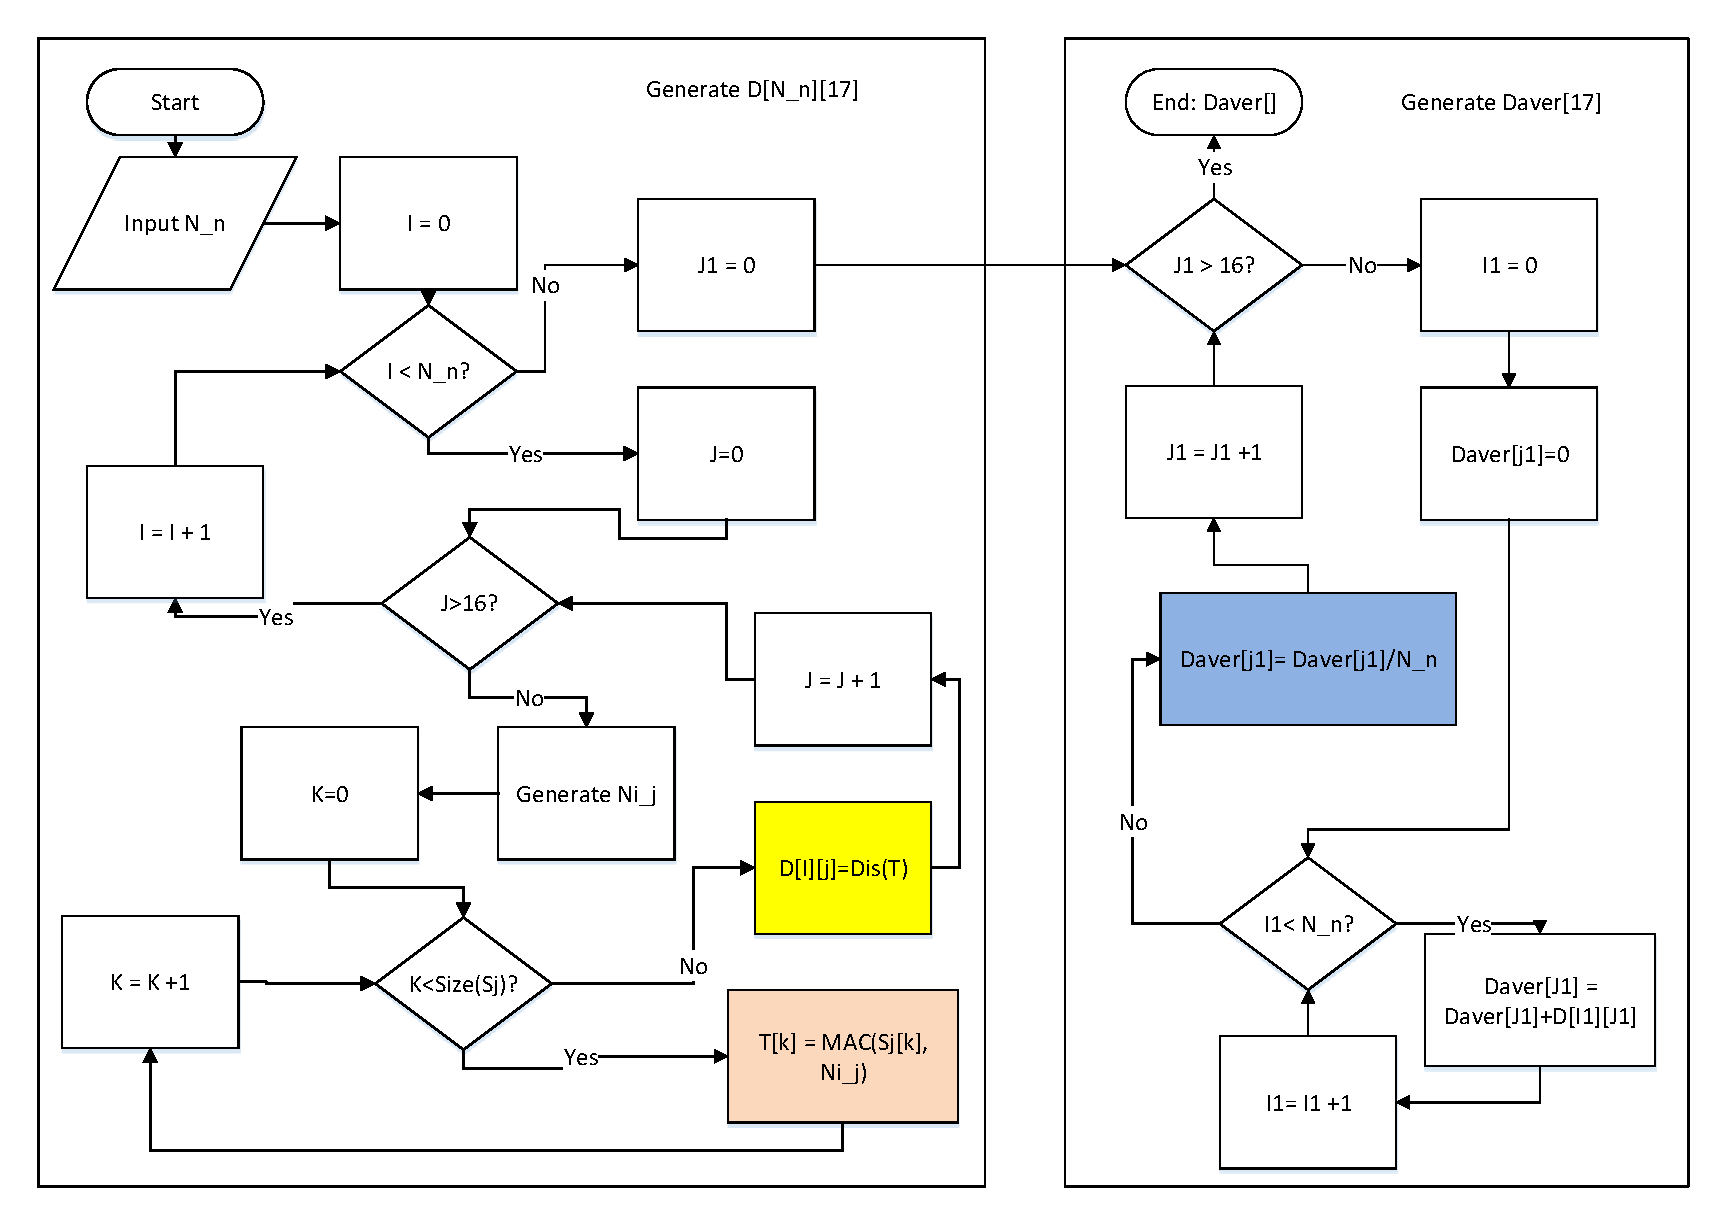
\includegraphics[scale=0.4]{./diagrams/nonceCollide.pdf}
 \caption{Simulation Flowchart of Content Modification Attack: Each element in Daver[17] is the average No. of distinct tags of set[i] under content modification attack, where i is the number of 1s in 16 bits}
 \label{fig:cma}
\end{figure}

We repeat the simulation 1000 rounds and compute the average of Round$_r$\_num\_T1\_S$_i$s and Round$_r$\_num\_T2\_S$_i$s seperately. The average results   Aver\_num\_T1\_S$_i$ and Aver\_num\_T2\_S$_i$ for each set S$_i$ serves as the indicator of the security of a tested scheme under content modification attack.
The concept of our simulation of content modification attack is expressed in Figure $\ref{fig:cma}$.

%input is fixed, nonce changes, No. of distinct tags
\subsubsection{Copying-then-Replaying Attack Simulation}
If the adversary conducts a copy-then-replay attack, he will maintain a copy of valid fram written in an older time point of on different memory address and then replace the vailid frame with this copy. This procedure can be modeled as querying the MAC scheme with a fixed chosen input while the input of nonce generation is distinct for each query. It is possible that two tags collide when they are generated with two distinct nonce but one identical input. The high probability of this collision indicates that the MAC scheme is unsecure under copy-then-replay attack.  

Our simulation of copy-then-replay attack is modeled into the following steps:
\begin{itemize}
	\item Step 1: Choose 0x0000 as the ciphertext 
	\item Step 2: Generate k tags with k nonces. The input to generation each nonce is distinct
	\item Step 3: Compute the No. of distinct tags among the k tags
	\item Step 4: If the ciphertext is not bigger than 0xFFFF, add it with one then repeat step 2 and step 3.
\end{itemize}
For each cip\begin{figure}[htbp]
 \centering
 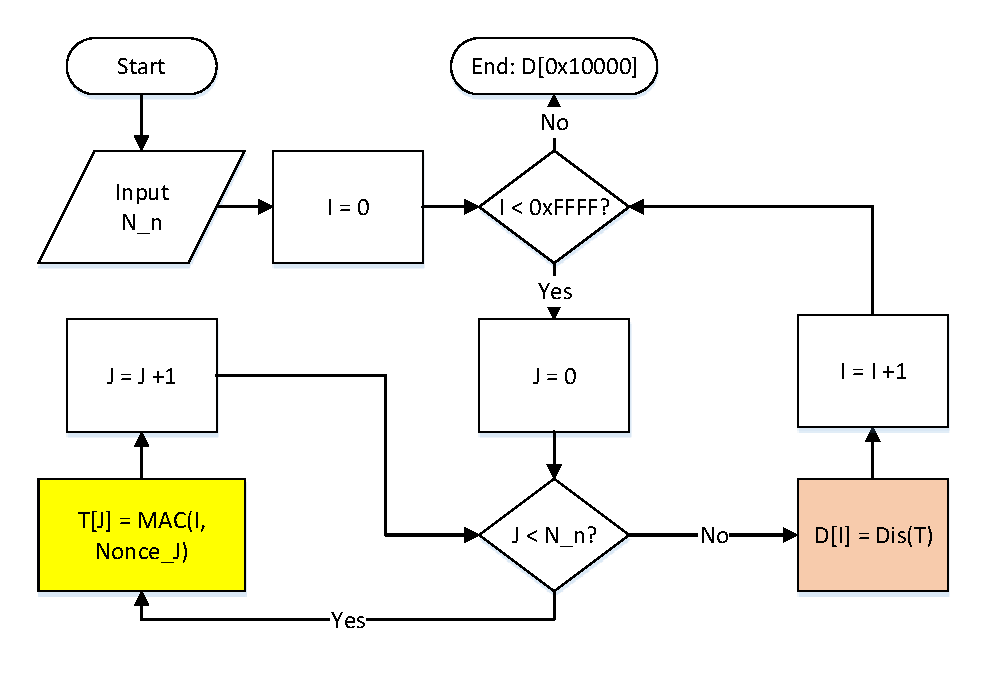
\includegraphics[scale=0.4]{./diagrams/replay_attack.pdf}
 \caption{Simulation Flowchart of Copy-then-replay Attack: Each element in D[0x10000] is No. of distinct tags of ciphertext i with 1000 different nonce under copy-then-replay attack, where i is the decimal value of a 16-bits ciphertext}
 \label{fig:ctra}
\end{figure}hertext, we generate 1000 tags. The concept of our simulation of copy-then-replay attack is also expressed in Figure $\ref{fig:ctra}$.
\end{document}
